\documentclass[11pt]{article}

\usepackage[a4paper,margin=2.25cm]{geometry}
\usepackage{amsmath,amssymb}
\usepackage{booktabs}
\usepackage{graphicx}
\usepackage{float}
\usepackage{hyperref}
\usepackage{siunitx}
\usepackage{microtype}
\graphicspath{{figures/}}

\title{Reproduction of Symbolic-Regression Reconstructions of Dark Energy Using DESI DR2 and Supernova Data}
\author{Keming Liu}
\date{17 October 2026}

\begin{document}

\maketitle

\begin{abstract}
We independently reconstruct the distance observables and dark-energy equation of state in Figures 1--3 of Sousa-Neto et al. (arXiv:2502.10506v2) using public DESI DR2, Pantheon+, and DES-SN5YR data. The DESI-only distance fit closely matches the published exponential family, and both combined-data sets admit exponential-family fits. Derived $w(z)$ intervals nevertheless depend on model choice and the treatment of pole-producing Monte Carlo draws. Several losses recalculated from the printed expressions do not match the reported values. We distinguish this unresolved numerical discrepancy from qualitative agreement and identify checks added in our reproduction.
\end{abstract}

\section{Scope and data}
\subsection{Three reconstruction tasks}
The target paper reconstructs $D_H/r_d$ from radial BAO data in Figure 1 and $D_M/r_d$ from transverse BAO plus supernova (SN) data in Figures 2 and 3~\cite{SousaNeto2025}. We use the six public DESI DR2 measurements of the relevant mode at $0.51\leq z\leq2.33$, extracting the corresponding $6\times6$ covariance submatrix from the 13-observable release matrix. The full DESI matrix is not diagonal: it contains within-bin $D_M$--$D_H$ correlations. The selected same-mode submatrices are diagonal. Fitting both modes jointly would be a different analysis from the paper's stated single-mode reconstruction.

\subsection{Supernova selection and distance conversion}
Following the reported cuts, Figure 2 combines six $D_M/r_d$ measurements with 1,590 Pantheon+ light curves at $z_{\rm HD}>0.01$ ($N=1596$). Figure 3 instead uses 1,754 DES-SN5YR objects with $\mathrm{MUERR\_FINAL}<1$ ($N=1760$). Both the fitted SN redshift and the factor $(1+z)$ below use $z_{\rm HD}$. For Pantheon+ we use corrected apparent magnitudes, $M=-19.253$, and nominal $r_d=138.28\,\mathrm{Mpc}$. For DES-SN5YR we use the released distance moduli and nominal $r_d=144.285714\,\mathrm{Mpc}$, corresponding to the stated $H_0=70\,\mathrm{km\,s^{-1}\,Mpc^{-1}}$ calibration. These nominal values prepare the SN distance vectors; the later $w(z)$ calculation uses the paper's $r_d=(101\pm2.3)\,h^{-1}\mathrm{Mpc}$ and fixed $\Omega_m=0.30$.

The common distance conversion and our first-order covariance propagation are
\begin{equation}
\mu=m_{b,\mathrm{corr}}-M\quad(\mathrm{Pantheon+}),\qquad
y\equiv\frac{D_M}{r_d}=\frac{10^{(\mu-25)/5}}{(1+z_{\rm HD})r_d},\qquad
C_y=JC_\mu J^T,\quad J_{ii}=\frac{\ln10}{5}y_i.
\label{eq:conversion}
\end{equation}
We use the public Pantheon+ STAT+SYS covariance, symmetrising its tiny numerical antisymmetry, and the DES-SN5YR systematic covariance plus statistical variances. Equation~\eqref{eq:conversion} retains off-diagonal SN correlations. The DESI--SN cross-survey covariance is assumed zero. The nominal $r_d$ is fixed during data preparation and varied as one shared calibration draw per Monte Carlo catalogue. The paper does not provide a fit-ready combined covariance matrix.

\section{Method and additions to the paper}
\subsection{Loss function and PySR configuration}
The paper states the covariance-weighted objective
\begin{equation}
\mathcal L=\frac{1}{N}(\boldsymbol y-\boldsymbol f)^T C^{-1}(\boldsymbol y-\boldsymbol f).
\label{eq:loss}
\end{equation}
We calculate it by a linear solve rather than explicitly forming $C^{-1}$. Table~\ref{tab:pysr} gives our recorded search settings. The operators follow those listed in the paper; the seed counts and search budgets are our implementation choices, not documented author settings. The paper-table DESI-error variant was used only for sensitivity checks.

\begin{table}[htbp]
\centering\small
\caption{PySR configuration used in this reproduction. The Figure 2 and 3 searches share the same settings but use different prepared data vectors and covariances.}
\label{tab:pysr}
\begin{tabular}{@{}p{4.2cm}p{5.0cm}p{5.0cm}@{}}
\toprule
Setting & Figure 1 & Figures 2 and 3\\
\midrule
Data and covariance & DESI $D_H/r_d$; public $6\times6$ submatrix & DESI $D_M/r_d$ + respective SN sample; public prepared covariance\\
Seeds & 100 deterministic targeted seeds & 100 deterministic seeds per scenario\\
Selection within each run & PySR \texttt{best} & PySR \texttt{best}\\
Maximum raw complexity & 7 & 9\\
Iterations; populations & 120; 8 & 30; 4\\
Population size; cycles/iteration & 30; 300 & 24; 100\\
Unary operators & $\log,\sqrt{\phantom z},\exp,\mathrm{square},\mathrm{cube}$ & Same\\
Binary operators & $+,-,\times,/,\mathrm{pow}$ & Same\\
\bottomrule
\end{tabular}
\end{table}

\subsection{Candidate selection}
The paper says PySR's \texttt{best} criterion first retains expressions below $1.5$ times the minimum error \emph{among all models}, then chooses the highest PySR score~\cite{SousaNeto2025}. For Figure 1, the paper-like exponential family is modal across our 100 public-covariance seeds (66/100); we refit its two coefficients by generalised least squares (GLS). For Figures 2--3, Notebook 11 applies our additional physical/numerical checks on $0\leq z\leq2.33$: finite distance, derivatives and $w$; $D_M(0)=0$; positive increasing distance; and a positive $w$-reconstruction denominator factor. It then keeps expressions whose original loss is at most $1.5$ times the minimum \emph{eligible} loss and chooses lowest raw complexity, breaking ties by loss and seed. The numerical factor $1.5$ comes from the paper/PySR rule, but applying it after our eligibility filter and then minimising complexity is \emph{not} the paper's selection algorithm. In Figure 2, 29 seed-selected expressions pass the physical checks and 26 remain after this loss gate. A simplified expression can have the continuous value $D_M(0)=0$ even when its unsimplified PySR tree contains $\log z$ and is undefined at exactly zero; we distinguish the two domains rather than claiming $\log 0$ is defined.

\subsection{From distance to the dark-energy equation of state}
We compute $w(z)$ using the paper's flat-universe relations. With $\widetilde D_H=D_H/r_d$, $\widetilde D_M=D_M/r_d$, and $\gamma=\Omega_mH_0^2r_d^2/c^2$,
\begin{align}
w_H(z)&=-1-\frac{2(1+z)\widetilde D_H'+3\gamma(1+z)^3\widetilde D_H^3}{3[\widetilde D_H-\gamma(1+z)^3\widetilde D_H^3]},\label{eq:wh}\\
w_M(z)&=-1-\frac{2(1+z)\widetilde D_M''+3\gamma(1+z)^3(\widetilde D_M')^3}{3[\widetilde D_M'-\gamma(1+z)^3(\widetilde D_M')^3]}.
\label{eq:wm}
\end{align}
\subsection{Monte Carlo uncertainty propagation}
The symbolic family remains fixed during Monte Carlo. Figure 1 uses 20,000 correlated DESI mock catalogues with GLS coefficient refits. Figures 2--3 initially used 10,000 first-order coefficient draws; a separate experiment used 20,000 correlated full-catalogue Gaussian mocks with fixed-family refits for each mock-centre choice. Each mock has one shared $r_d$ calibration draw. These intervals include coefficient and calibration uncertainty conditional on the selected family, but not uncertainty from rerunning PySR.

We report all finite draws and, separately, draws without a grid-bracketed zero of the $w$ denominator. The latter is a conditional subset. Bands are pointwise quantiles, not simultaneous confidence bands. These Monte Carlo and pole-screening specifications are our additions; the paper does not fully document its resampling procedure.

\section{Results: printed formulae versus independent fits}
\subsection{Published expressions and independent fits}
The paper's Appendix A lists candidate expressions in Tables III--V; its main text also gives Eqs.~(10), (12), and (13). Table~\ref{tab:printed} evaluates the specified printed forms as written. A reported loss is shown only where it accompanies that exact selected table row; a dash indicates no separately published loss for the alternative rendering. Table~\ref{tab:ourfits} contains our fits.

\begin{table}[htbp]
\centering\small
\caption{Published expressions, evaluated literally with our prepared public data and Eq.~\eqref{eq:loss}. ``Reported'' is populated only where the paper prints a loss beside the selected row in Appendix A. The full candidate lists remain in the paper's Tables III--V.}
\label{tab:printed}
\begin{tabular}{@{}clp{5.0cm}rr@{}}
\toprule
Fig. & Printed location & Expression as printed & Reported & Recomputed\\
\midrule
1 & Table III, selected & $28.42/1.68^z$ & 0.30 & 0.664\\
  & Main-text Eq.~(10) & $28.4e^{-0.519z}$ & --- & 0.704\\
\addlinespace
2 & Table IV, selected$^{\dagger}$ & $0.76^{2}z/0.03$ & 1.70 & 21.333\\
  & Appendix Eq.~(A2) & $0.76^{z}z/0.03$ & --- & 4.789\\
  & Main-text Eq.~(12) & $33.3ze^{-0.274z}$ & --- & 4.729\\
\addlinespace
3 & Table V, selected & $30.1z/1.31^z$ & 2.23 & 0.990\\
  & Appendix Eq.~(A3) & $30.1z/1.30^z$ & --- & 1.015\\
  & Main-text Eq.~(13) & $30.1ze^{-0.262z}$ & --- & 1.016\\
\bottomrule
\end{tabular}
\par\smallskip\footnotesize $^{\dagger}$The exponent $2$ is reproduced literally from Table IV and is likely a typographical error: Appendix Eq.~(A2) instead gives exponent $z$. The two forms have different recomputed losses.
\end{table}

\begin{table}[htbp]
\centering\small
\caption{Our fits, distinguished from published expressions. Figure 2's later re-ranking was exploratory and does not replace the original Notebook 11 selection.}
\label{tab:ourfits}
\begin{tabular}{@{}clp{6.5cm}r@{}}
\toprule
Fig. & Our analysis & Independent/refitted expression & Our $\mathcal L$\\
\midrule
1 & PySR family, GLS refit & $28.120223e^{-0.508294z}$ & 0.407\\
2 & Initial independent selection & $z(28.997298-5.714456z)$ & 0.920\\
2 & Exploratory re-ranking of same seeds & $29.321837ze^{-0.250232z}$ & 0.884\\
3 & Independent selection & $29.438630z/1.295185^z$ & 0.937\\
\bottomrule
\end{tabular}
\end{table}
\clearpage

\subsection{Figure 1: DESI-only reconstruction}
\begin{figure}[H]
\centering\IfFileExists{figures/fig1_mc.png}{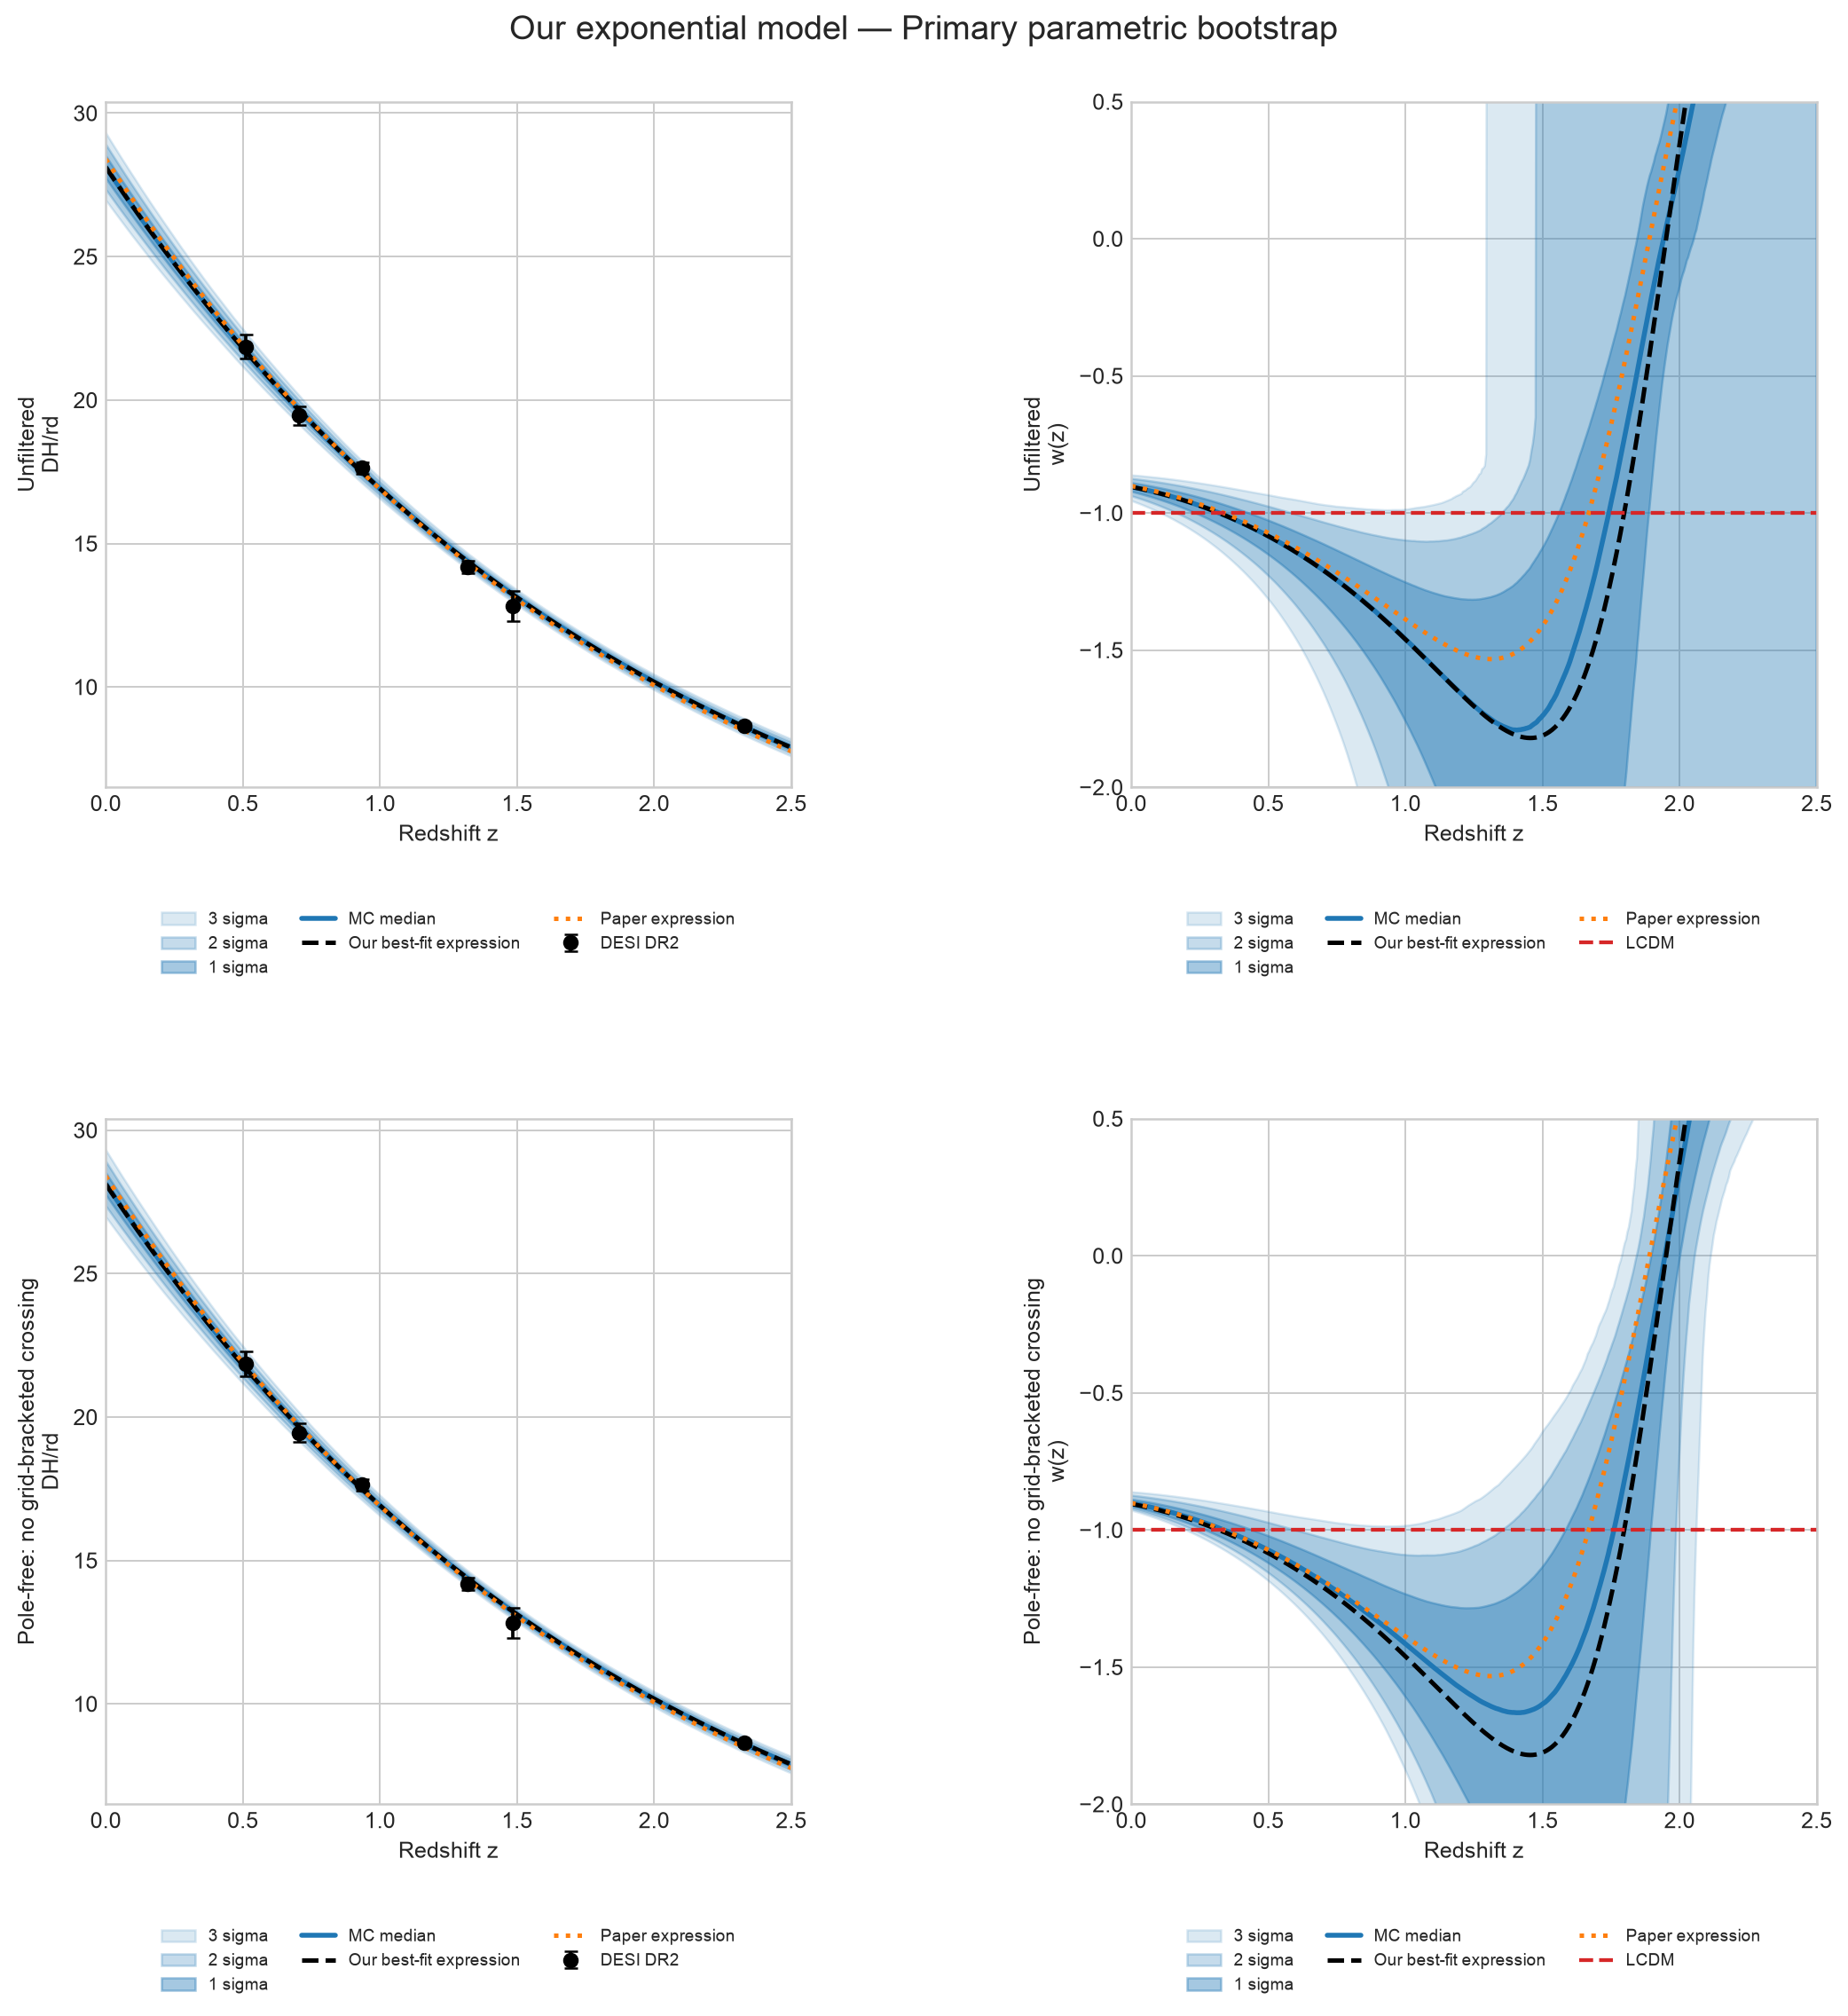
\includegraphics[width=0.73\linewidth]{figures/fig1_mc.png}}{\fbox{Figure 1 plot: upload figures/fig1\_mc.png}}
\caption{Our Figure 1 reconstruction, with the paper's \emph{printed formula} drawn for comparison. Top: all finite draws; bottom: pole-free subset. Compare the authors' published Figure 1 in Ref.~\cite{SousaNeto2025}; their confidence bands need not share our Monte Carlo definition.}
\label{fig:fig1}
\end{figure}
The independent and main-text paper distance curves differ by at most approximately $1.7\%$ over $0\leq z\leq2.5$; nevertheless, Eq.~(10) itself has recomputed loss 0.704, rather than the Table III selected-row value of 0.30. Differentiation and the denominator in Eq.~\eqref{eq:wh} amplify the small distance-level difference in $w(z)$. Of 20,000 model-centred mocks, 16,895 are pole-free on the tested grid. In this conditional subset $w=-1$ lies outside our pointwise $3\sigma$ interval below approximately $z=0.20$; without pole filtering the low-$z$ boundary is nearer $0.11$. Both boundaries lie below the lowest DESI measurement, $z=0.51$: this is extrapolation of the fitted family, not direct low-redshift evidence against $\Lambda$CDM. The published confidence-band boundaries are not reproduced exactly.

\clearpage
\subsection{Figure 2: DESI and Pantheon+ reconstruction}
\begin{figure}[H]
\centering\IfFileExists{figures/fig2_mc.png}{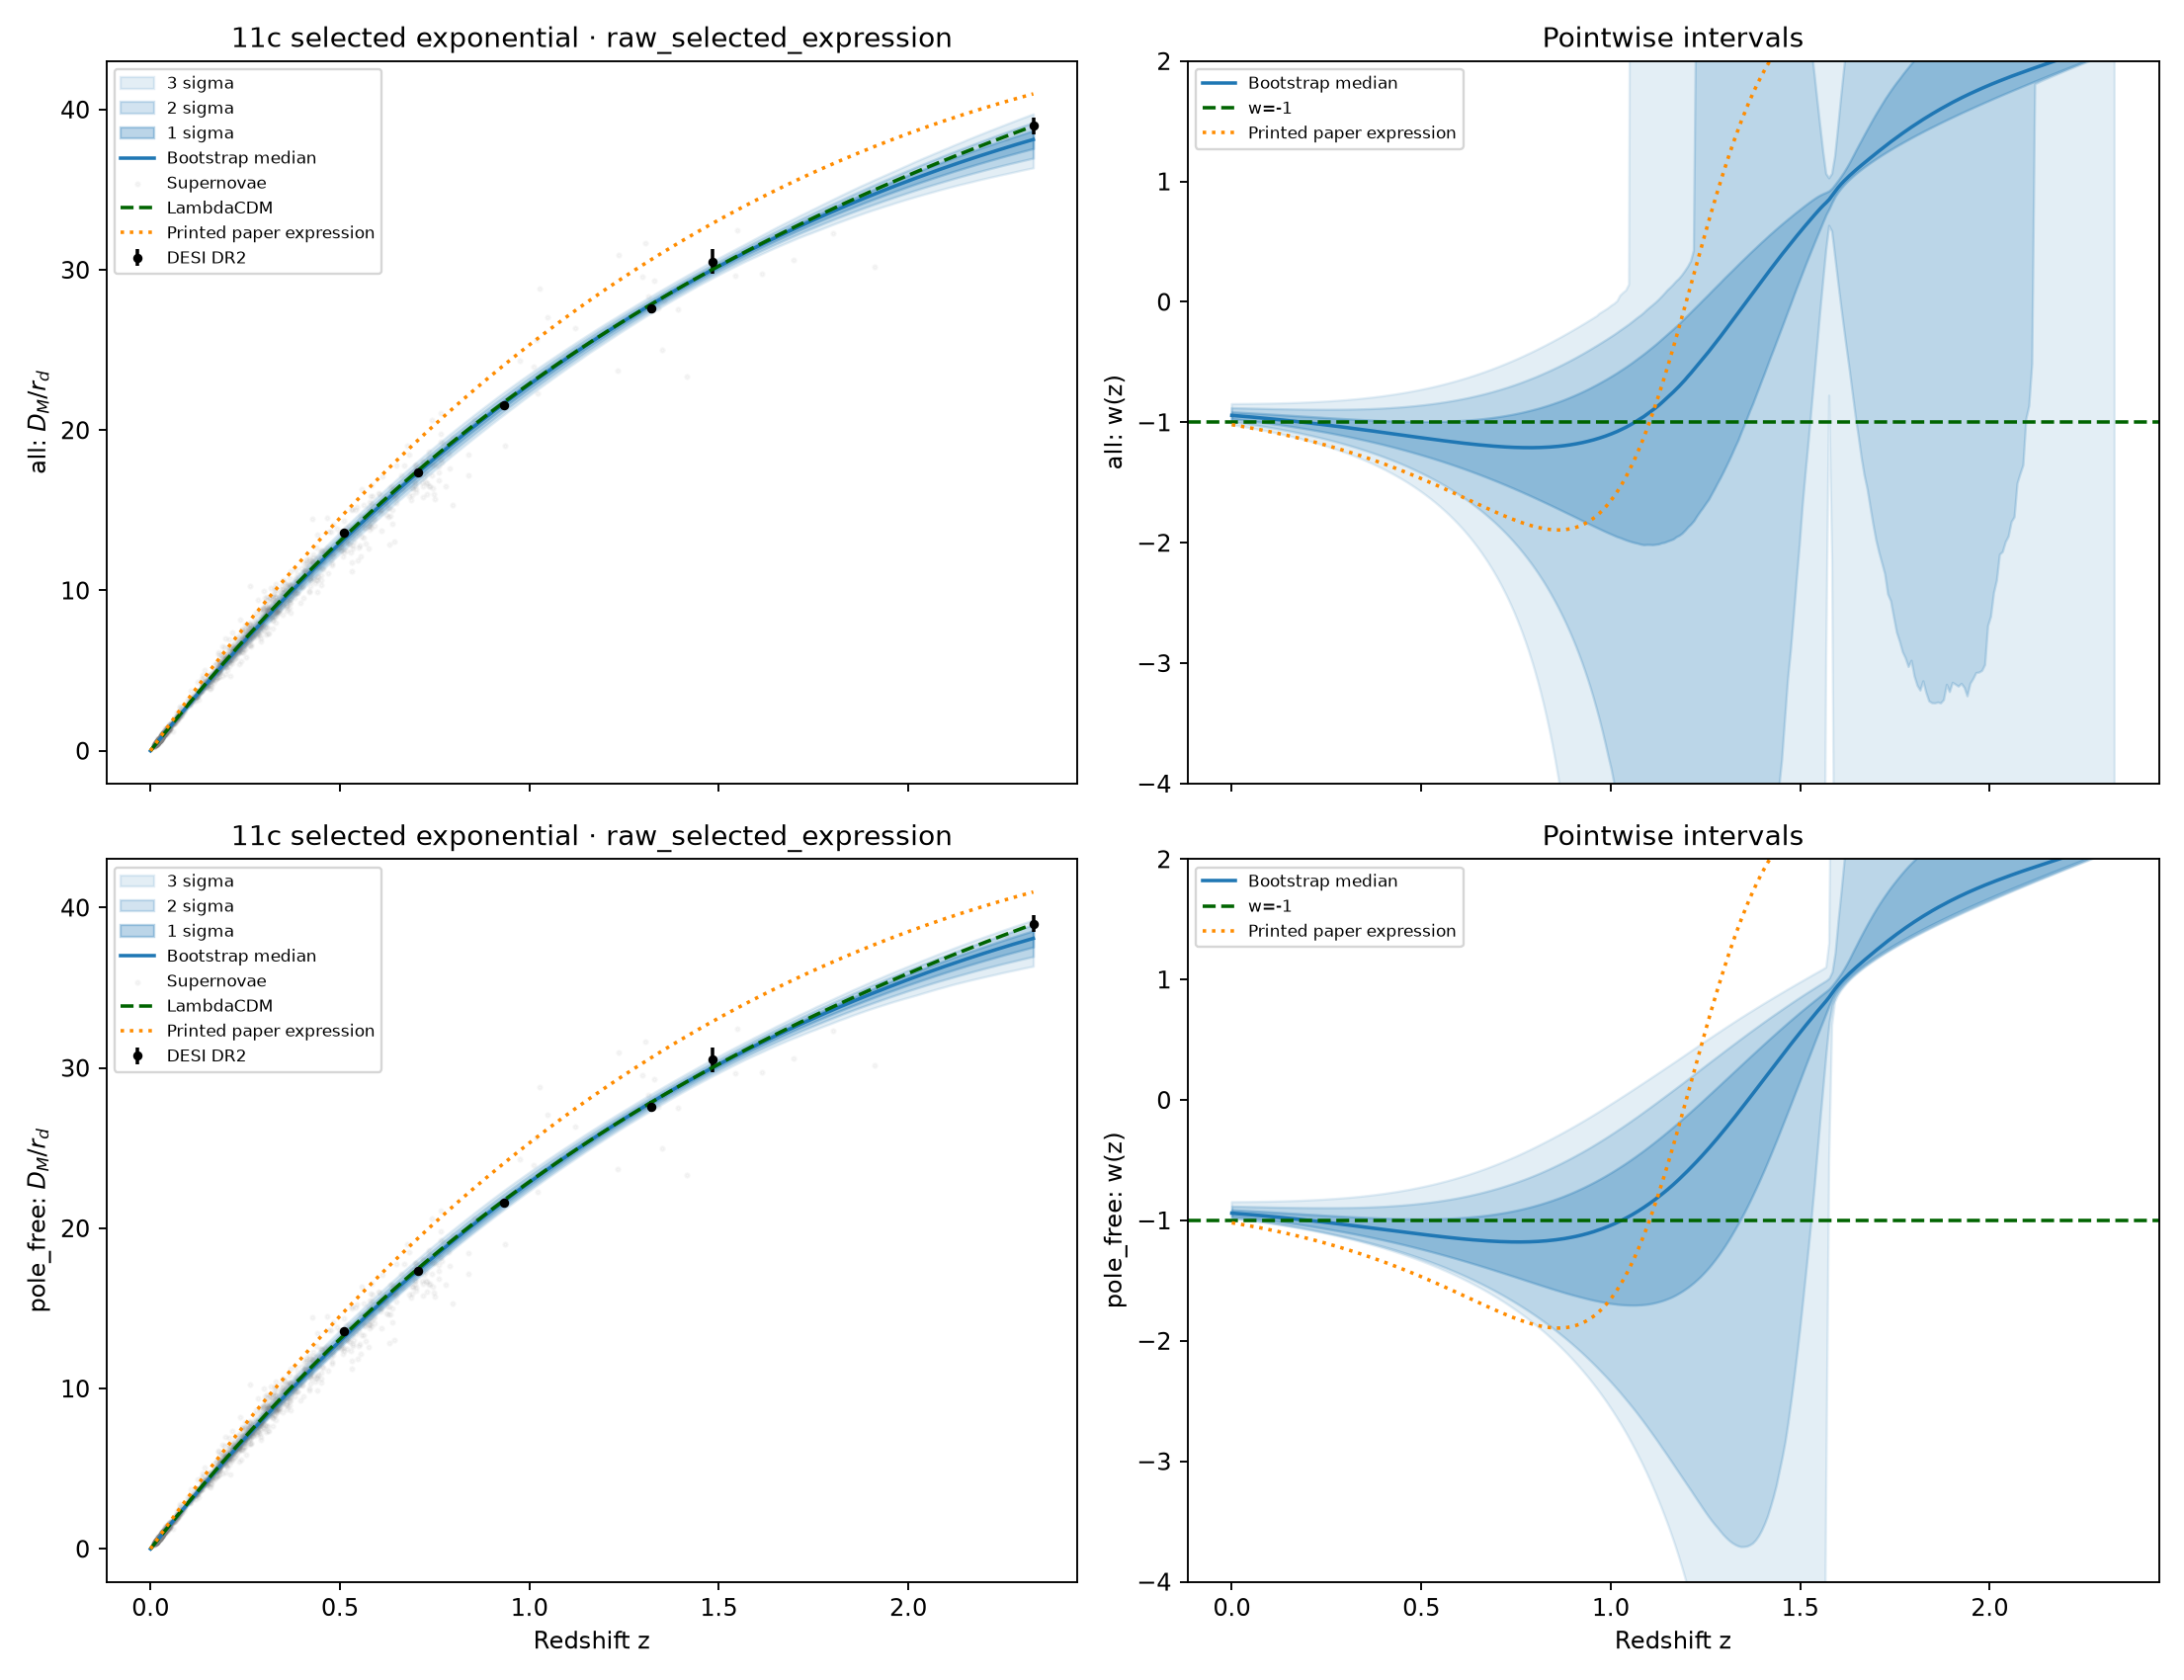
\includegraphics[width=0.80\linewidth]{figures/fig2_mc.png}}{\fbox{Figure 2 plot: upload figures/fig2\_mc.png}}
\caption{Our exploratory Figure 2 exponential and the printed Eq.~(12) curve (orange dotted), with full-catalogue Monte Carlo bands. Top: all finite draws; bottom: pole-free subset. The authors' published Figure 2 is in Ref.~\cite{SousaNeto2025}, but its uncertainty procedure is not fully specified.}
\label{fig:fig2}
\end{figure}
Our original independent lowest-complexity choice was quadratic. Its combined loss of 0.920 looked acceptable, but a frozen-fit residual audit separated the six BAO points from the 1,590 SNe: $\chi^2_{\rm DESI}/6=6.988$ versus $\chi^2_{\rm SN}/1590=0.897$. Because the SN sample is much larger, its good fit can dominate the combined average; a low joint loss does not guarantee a good BAO fit. This diagnoses a weakness of \emph{this selected quadratic}, not of all quadratics.

After observing this imbalance, Notebook 11c \emph{exploratorily} re-ranked the existing 100-seed catalogue, minimising the worse of the two subset scores while retaining Notebook 11's eligibility and joint-loss gate. It selected seed 20261093's actual PySR exponential, with $\chi^2_{\rm DESI}/6=1.714$, $\chi^2_{\rm SN}/1590=0.881$, and combined loss 0.884. This is neither a manual fit to the paper's coefficients nor the original blinded selection. The exact structure appeared in only one seed-selected result, so it is not a stable recovery claim. Its raw PySR tree has complexity 9, though the displayed simplified expression has seven default-count nodes; complexity attaches to the search tree, not automatically to the later algebraic simplification.

In 20,000 model-centred full-catalogue refits of this fixed exponential family, 18,522 are pole-free. The all-draw pointwise $3\sigma$ $w$ interval includes $-1$ at all reported checkpoints except one isolated grid point; the pole-free interval excludes $-1$ near $z=0$ and at high $z$. These are different conditional ensembles. Neither isolated crossings nor filtered pointwise intervals establish a global rejection of $\Lambda$CDM.

\clearpage
\subsection{Figure 3: DESI and DES-SN5YR reconstruction}
\begin{figure}[H]
\centering\IfFileExists{figures/fig3_mc.png}{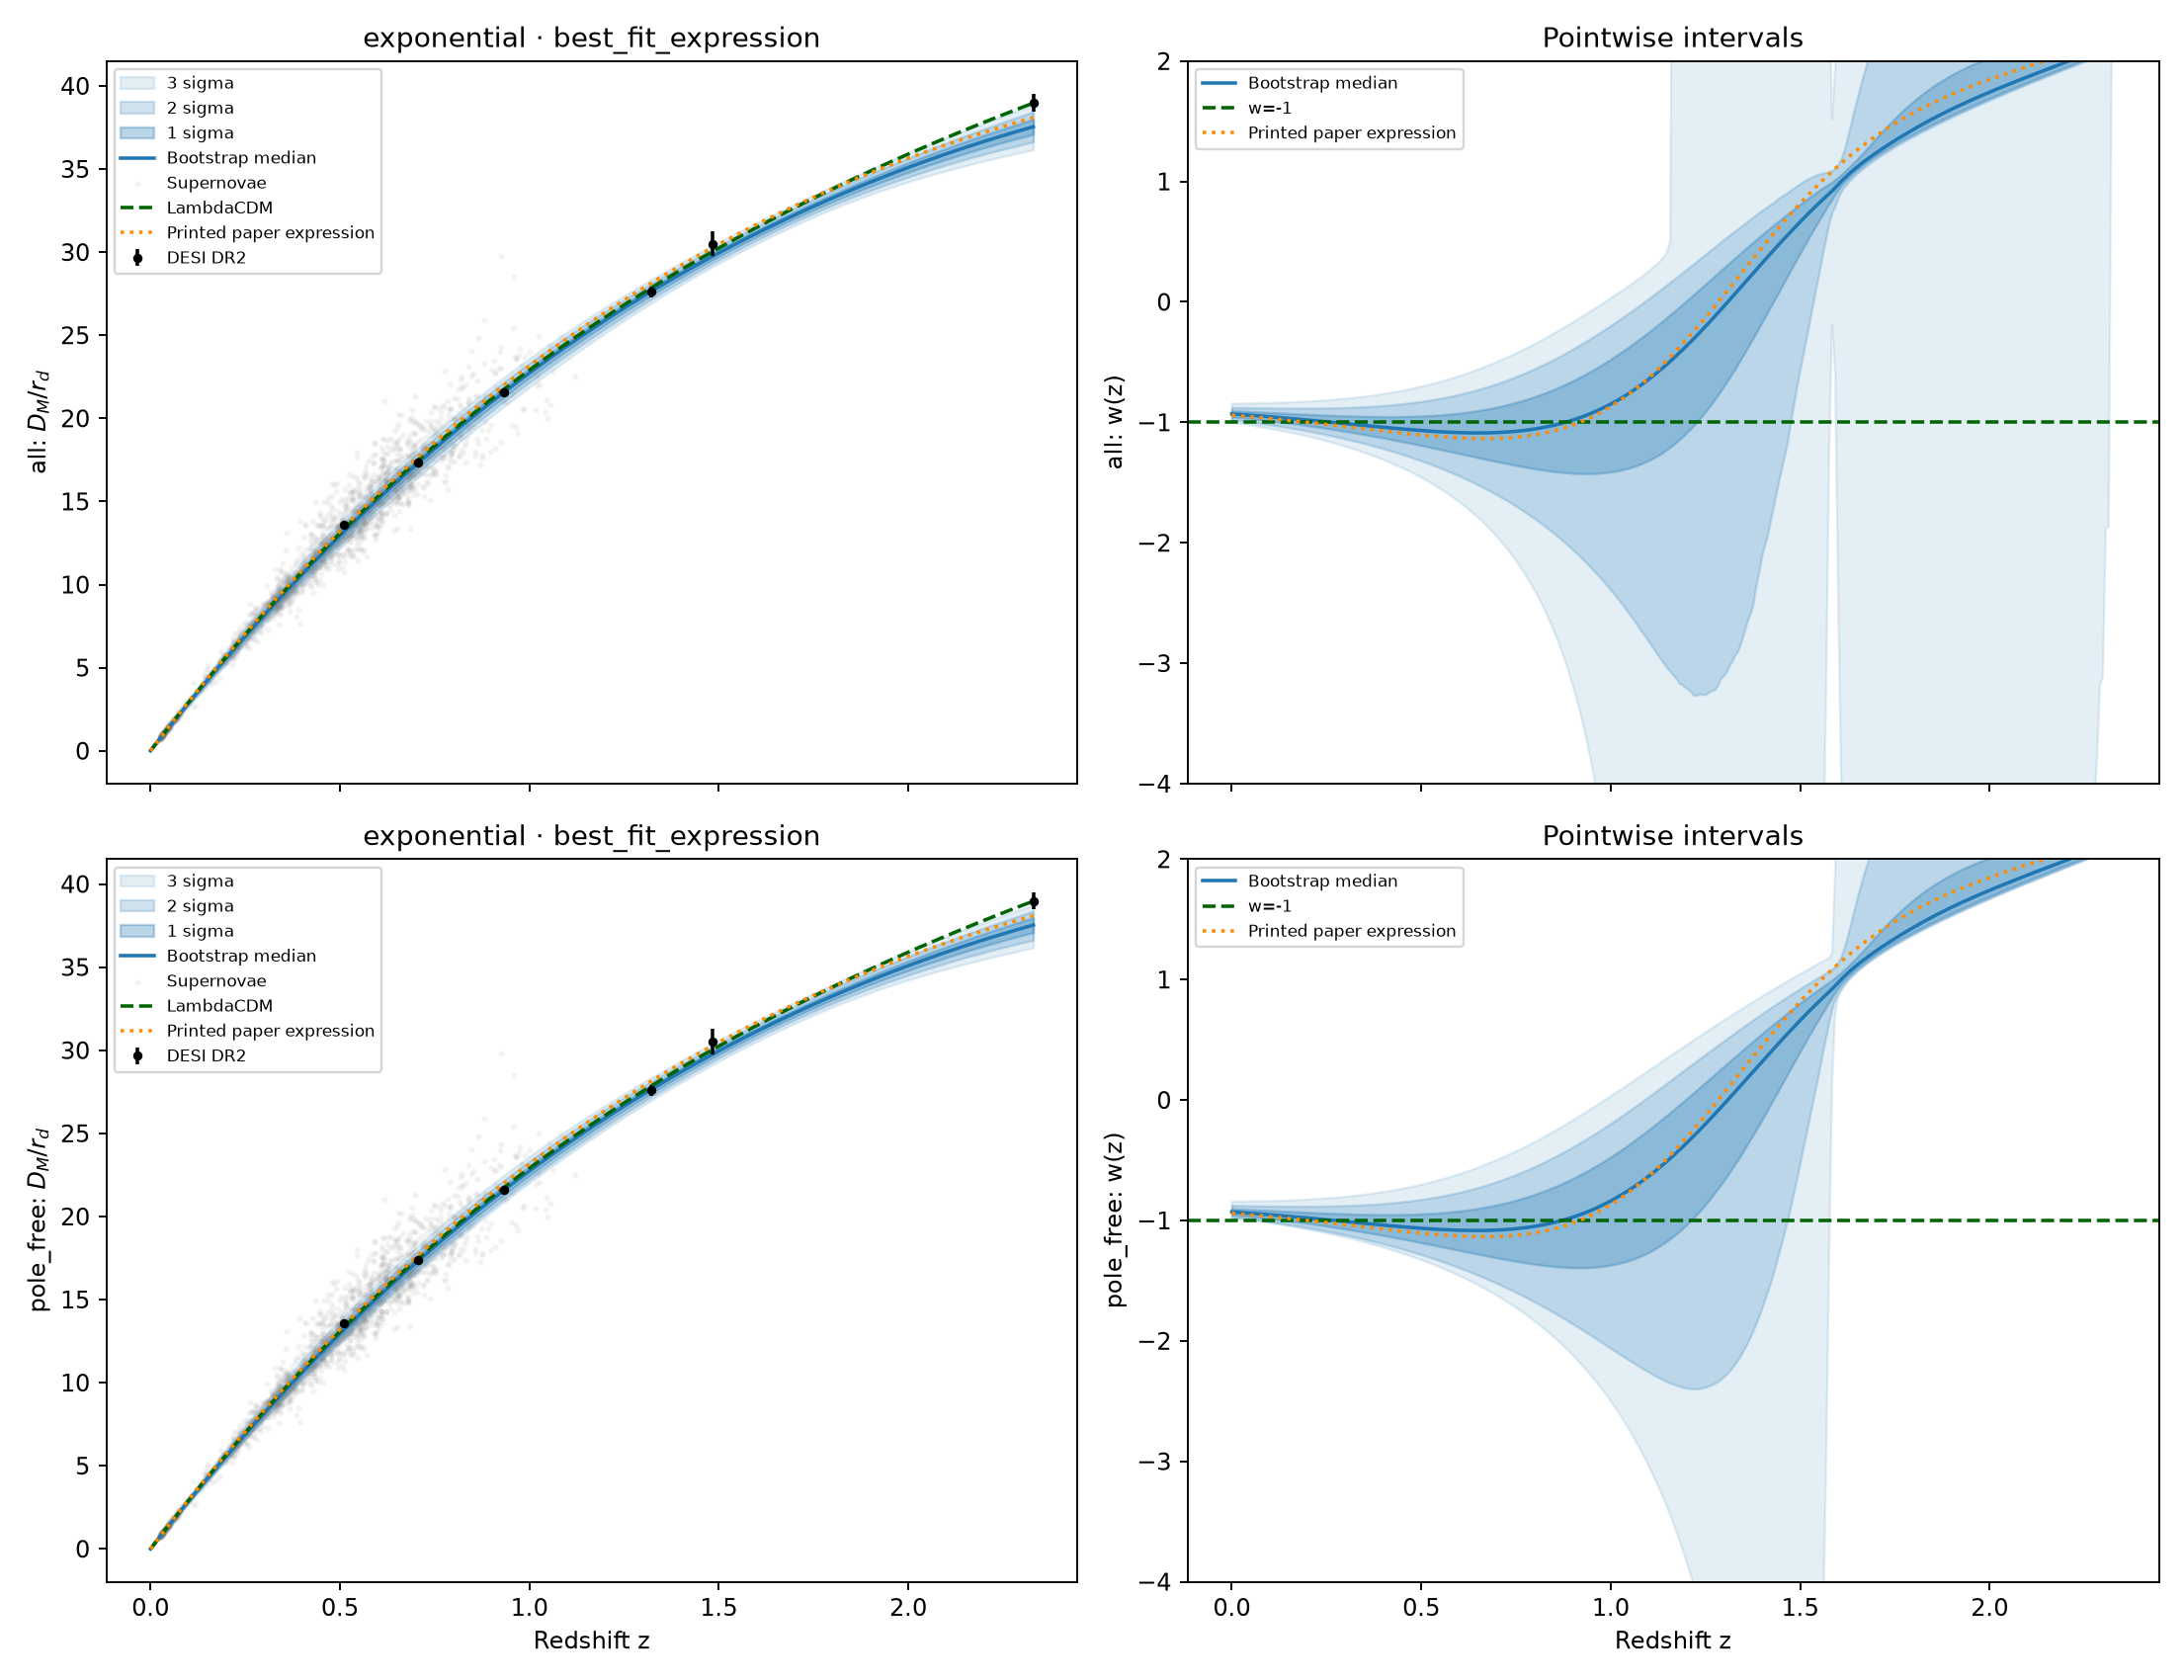
\includegraphics[width=0.80\linewidth]{figures/fig3_mc.png}}{\fbox{Figure 3 plot: upload figures/fig3\_mc.png}}
\caption{Our Figure 3 independent exponential, with the paper's printed expression overlaid. Top: all finite draws; bottom: pole-free subset. The authors' Figure 3 can be consulted separately in Ref.~\cite{SousaNeto2025}.}
\label{fig:fig3}
\end{figure}
The original independent choice was already exponential; no later structural re-selection was needed. Its combined loss is 0.937, with $\chi^2_{\rm DESI}/6=2.486$ and $\chi^2_{\rm SN}/1754=0.932$. Of 20,000 model-centred full-catalogue refits, 19,640 are pole-free. Its pole-free interval at $z=0$ excludes $w=-1$, but this endpoint statement depends on the fixed family and the pole selection, and is not a global rejection of $\Lambda$CDM. Individual BAO residuals remain non-negligible despite the satisfactory joint average.

\section{Published-loss discrepancies}
\subsection{Differences among printed expressions}
The selected row of Table IV literally prints $0.76^{2}z/0.03$; Appendix Eq.~(A2) gives $0.76^{z}z/0.03$, and main-text Eq.~(12) is the rounded exponential $33.3ze^{-0.274z}$~\cite{SousaNeto2025}. The exponent-2 and exponent-$z$ versions are different functions, not merely different typography. Table~\ref{tab:printed} shows why one cannot automatically attach Table IV's reported 1.70 to the exact main-text rendering. Figure 3 likewise has a small printed-base difference between Table V ($1.31^z$) and Appendix Eq.~(A3) ($1.30^z$). We retain each source location explicitly rather than silently choosing one as the authors' hidden fit.

\subsection{Sensitivity checks and unresolved inputs}
A candidate-by-candidate audit of Tables III--V found that some printed candidates approximately match their reported losses but others do not. We tested public versus paper-table DESI errors, full versus diagonal covariance, Pantheon+ STAT+SYS versus STATONLY, alternative SN redshift columns, nominal calibration changes, alternative objectives, and variation of printed constants restricted to their rounding intervals. None consistently reconciles all selected rows and candidates. Rounding contributes for some sensitive expressions but is not a complete explanation. Because Figure 1 also disagrees without SN conversion, the SN covariance Jacobian cannot be the \emph{common} cause across all three figures. The authors' full-precision expressions, exact fit-ready vectors, or code would be needed to establish the provenance of their reported losses; we do not claim to have identified a single cause.

\section{Assessment and limitations}
We reproduce the broad distance-level trends and obtain independent interpretable expressions in all three scenarios, but not every printed coefficient, loss, or confidence band. The Figure 2 subset audit demonstrates why both the combined and survey-specific residuals matter. Derived $w(z)$ is more sensitive than the fitted distances to the selected functional family, differentiation, extrapolation, calibration, and denominator poles. Our pointwise intervals are conditional reconstructions, not tests that globally establish or exclude $\Lambda$CDM. The notebook sequence and timestamped result folders preserve each input version and independent or exploratory decision; the \href{https://app.notion.com/p/dbe79fe1f4924b4ba836b4b8a788eee6}{research log} records their chronology.

\appendix
\section{Eligible PySR candidate expressions}
Table~\ref{tab:fig2candidates} and Table~\ref{tab:fig3candidates} cover all 29 seed-selected expressions per combined-data scenario that passed the Notebook 11 physical and numerical checks. Algebraically equivalent or nearly identical fits are grouped; displayed coefficients are rounded, whereas all selection losses used the saved full-precision expressions. Seed labels omit the common prefix \texttt{2026} (for example, \texttt{1012} denotes seed \texttt{20261012}). These are \emph{our} PySR candidates, not the published Appendix A candidates. The complete, ungrouped expressions and diagnostics are preserved in each scenario's \texttt{candidate\_diagnostics.csv} file under \texttt{results/11\_fig23\_mc\_and\_reconstruction/}.

\begin{table}[htbp]
\centering\scriptsize
\caption{Figure 2: 29 eligible seed-selected candidates, grouped by approximate algebraic form. Losses are recomputed using the prepared public covariance.}
\label{tab:fig2candidates}
\begin{tabular}{@{}p{4.8cm}p{7.5cm}r@{}}
\toprule
Representative $D_M/r_d$ & Seeds (prefix \texttt{2026} omitted) & Loss\\
\midrule
$z(28.9973-5.7145z)$ & 1012, 1014, 1016, 1020, 1023, 1027, 1036, 1044, 1052, 1053, 1054, 1057, 1058, 1064, 1076, 1078, 1085, 1088, 1089, 1095, 1096, 1097, 1103 & $\simeq0.920$\\
$z(28.6616-5.4754z)$ & 1043 & 0.943\\
$5.3954z(5.3444-z)$ & 1083 & 0.928\\
$z/[0.0188245(z+1.67874)]$ & 1031 & 1.692\\
$50.5887z/(z+1.57677)$ & 1062 & 1.896\\
$57.1972z/(z+1.79051)$ & 1075 & 1.609\\
$29.32184z/1.284323^{z}$ & 1093 & 0.884\\
\bottomrule
\end{tabular}
\end{table}

\begin{table}[htbp]
\centering\scriptsize
\caption{Figure 3: 29 eligible seed-selected candidates, grouped as in Table~\ref{tab:fig2candidates}.}
\label{tab:fig3candidates}
\begin{tabular}{@{}p{4.8cm}p{7.5cm}r@{}}
\toprule
Representative $D_M/r_d$ & Seeds (prefix \texttt{2026} omitted) & Loss\\
\midrule
$z(28.7725-5.6766z)$ & 1014, 1015, 1022, 1025, 1026, 1028, 1034, 1038, 1040, 1042, 1046, 1052, 1059, 1062, 1067, 1081, 1088, 1093, 1094, 1095, 1099 & $\simeq0.982$\\
$29.43863z/1.295185^{z}$ & 1011, 1023, 1036, 1047, 1101 & 0.937\\
$29.13172z/1.280609^{z}$ & 1079 & 0.944\\
$z(z-8.7979)^2/2.6568$ & 1035 & 0.955\\
$z(3.0824-z/4.0586)^3$ & 1054 & 0.948\\
\bottomrule
\end{tabular}
\end{table}

\section*{AI use declaration}
I used OpenAI Codex/ChatGPT to assist with code development and debugging, methodological discussion, LaTeX drafting and editing, and presentation of the results. Numerical claims in this report are tied to saved notebook outputs and public-data checks; AI-generated suggestions were not treated as independent evidence. I remain responsible for the data choices, interpretation, and any remaining errors. Unresolved differences from the paper are stated explicitly rather than filled in by AI inference.

\begin{thebibliography}{9}
\bibitem{SousaNeto2025} A. Sousa-Neto, C. Bengaly, J. E. Gonzalez, and J. Alcaniz, \emph{Evidence for dynamical dark energy from DESI-DR2 and SN data? A symbolic regression analysis}, arXiv:2502.10506v2 (2025), \url{https://arxiv.org/html/2502.10506v2}.
\bibitem{DESI} DESI Collaboration, public DR2 BAO measurements and covariance, \url{https://github.com/CobayaSampler/bao_data}.
\bibitem{Pantheon} Pantheon+SH0ES Collaboration, public Pantheon+ data release, \url{https://github.com/PantheonPlusSH0ES/DataRelease}.
\bibitem{DESY5} DES Collaboration, public DES-SN5YR data release, \url{https://github.com/des-science/DES-SN5YR}.
\end{thebibliography}

\end{document}
